\section{Introduksjon}\label{sec:intro}

Analog motorlab hadde som mål å konstruere et sett med kretser for å måle og kontrollere en servomotor. Disse kretsene var delt inn i 4 forskjellige delsystemer, hastighetsmåler, hastighetsregulator, posisjonsmåler og posisjonsregulator, som vist i \autoref{fig:blokkdiagram}. Denne rapporten vil gå gjennom teori, metode, resultater og diskusjon for hver av delsystemene.

Utlevert til labratoriearbeidet var et motorkort og et studentkort, motoren med tachometeret og potensiometeret var koblet på et ferdig montert motorkort som ga tilgang til informasjon om motorens hastighet $\omega$ og posisjon $\theta$. Studenkortet besto av 13 operasjonsforsterkerer av typen LM741\cite{LM741} og et sett med header-pinner for å koble til motorkortet med. Operasjonsforsterkerene ble alle forsynt med $\pm${\SI{15}{\volt}}. Motorens hastighet kunne justeres ved å endre spenningen $V_m$ på en en av pin headerene. Det ble først laget et system for å måle og regulere hastighet før det ble laget et tilsvarende system for å måle og regulere posisjonenen til motoren.

\begin{figure}[bh]
    \centering
    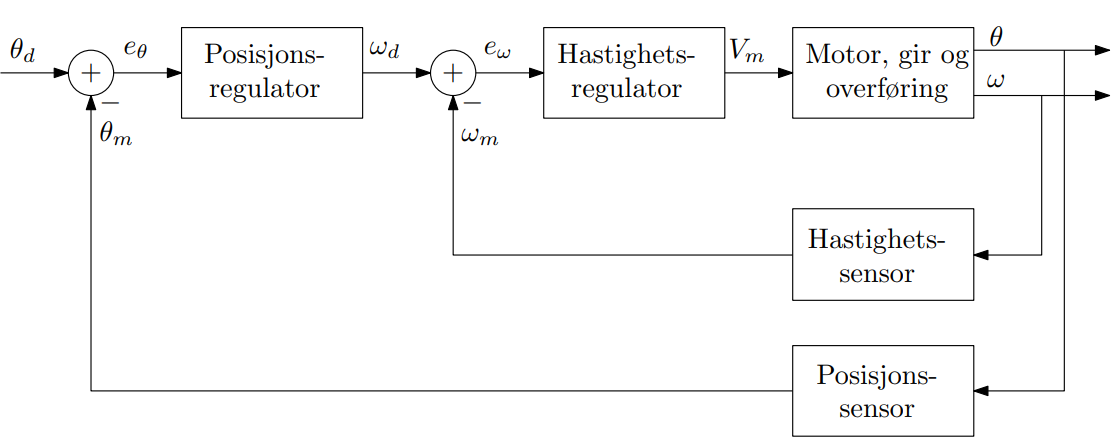
\includegraphics[width = 0.5\textwidth]{figurer/Blokkdiagram.png}
    \caption{Blokkdiagram over servomotoren. Diagramet viser regulatorene og signalomforming. Diagrammet er hentet fra \cite{AnalogMotorlabbOppgaver}}
    \label{fig:blokkdiagram}
\end{figure}

% Introduksjonen skal inneholde en oversikt over arbeidet dere har gjort, samt noen setninger som gir en videre kontekst for arbeidet (hva er nytten av å gjøre det dere har gjort i den store sammenhengen?). Dere kan også gjerne gi en kort beskrivelse av hvordan rapporten er organisert.

% Dere bør selvsagt legge mest fokus på å gjøre godt arbeid på labben, og å
% presentere det dere har gjort. Når det er sagt, er både innhold og
% presentasjon viktig. Husk at rapporten er deres eneste mulighet til å vise
% frem innsatsen dere har gjort, og hvordan dere legger det frem er derfor
% viktig. Hvis arbeidet dere har gjort på labben er fantastisk, men dere ikke
% klarer å formidle det i rapporten, så er det lite sannsynlig at dere får 
% uttelling for det. En figur som viser hvor bra regulatoren deres fungerer
% har liten verdi dersom den mangler en skikkelig beskrivelse av hva som blir
% vist. Husk også at gode diskusjoner av resultatene er viktig for å vise frem
% at dere forstår hva dere har gjort, og hvordan systemet fungerer.

% Layout er mindre viktig enn innhold, men det er fortsatt viktig. Dere kan
% tenke på rapportskriving som å skulle selge en leilighet; når du har 
% visning har du selvsagt vasket og ryddet for at den skal se så fin ut som
% mulig. Hvor ren leiligheten er avgjør selvsagt ikke verdien til leiligheten,
% men den påvirker hvilken subjektiv verdi kjøperne setter på leiligheten.
% På samme måte vil en rapport som ser pen og ryddig ut være enklere å lese, 
% og det er større sannsynlighet for at leseren får med seg det dere prøver å
% formidle.

% \subsection{Programvare}
% Dere står fritt til å velge programvare for rapportskriving.
% Dere kan for eksempel bruke Word eller andre tilsvarende programmer. 
% Ulempen med slike programmer er at det ofte er vanskelig (og av og til umulig)
% å få en god layout. Støtte for vektorgrafikk (forklares mer senere) er dårlig,
% og teksten ser sjelden like bra ut. På toppen av dette er det både vanskeligere
% å inkludere matematiske uttrykk, og resultater blir sjelden bra. Generelt vil 
% en rapport skrevet i Word ligne mer på et utkast enn en endelig rapport.

% Å bruke \LaTeX er sterkt anbefalt. Da er du nesten garantert at rapporten ser 
% bra ut, med mindre du gjør store endringer på konfigurasjonen. Det kan ta litt tid
% å komme i gang, men dere vil få utbytte av denne innsatsen både mot slutten av 
% rapportskrivingen, samt i senere fag og på masteroppgaven. \LaTeX har også 
% utmerket støtte for både matematiske uttrykk og vektorgrafikk.
